\chapter{Udviklingsmodel - Scrum}
Under dette projektforløb er scrum udviklingsmodellen brugt til processtyring. Denne udviklingsmodel er en iterativ metode der bruges til styring, organisering og planlægning af produkt udviklingen.

%I dette afsnit beskrives den udviklingsmodel der anvendes i forbindelse projektets forløb. I dette projekt er der blevet gjort brug af scrum som udviklingsmetode.

\section{Rollebeskrivelser}
Der er tre hovedroller i scrum; produktejeren, udviklingsholdet og scrum masteren. Disse tre roller udgør scrumteamet. Under dette projekt har gruppevejlederen fungeret som produktejeren, udviklingsholdet har bestået af projektgruppen og rollen som scrum master er skiftevis varetaget af forskellige medlemmer af gruppen.

\subsection{Produktejer}
Når der udvikles et produkt er der som regel en produktejer, der har stor interesse i det endelige produkt. Produktejeren definerer rammerne omkring produktet og prioriterer vigtigheden af opgaver på backloggen. \newline

I dette projektforløb er rollen som produktejer en kunstig rolle, i den forstand at gruppen har sat rammerne omkring projektet og prioriterer opgaver under forløbet. Gruppens vejleder har påtaget sig rollen som produktejer, men har meget lidt indflydelse på udkommet af projektet. Til sprintenes afslutningsmøder fungerede vejlederen som en konventionel produktejer. Her blev resultaterne af sprintet fremført for produktejeren, som skulle forholde sig kritisk i forhold til resultaterne.

Under et sprintplanlægningsmøde havde produktejeren en reel indfyldelse på prioritering af opgaver, og opgaverne på sprintbackloggen. Inden mødet med produktejeren havde gruppen afholdt et møde og udvalgt de vigtigste opgaver til sprintet. Herefter blev mødet med produktejeren afholdt, som hjalp med prioriteringen af opgaverne og gav forslag til opgaver, der ikke var taget højde for.  

Vejlederens forudsætning for at prioritere de opgaver, der skulle løses i det kommende sprint var at prioritere de læringsmål, der er opstillet i kursusbeskrivelsen \ref{laeringsmaal}. Det var altså vejlederens opgave at vejlede gruppen, så der ved afslutningen af projektet ville være opfyldt så mange læringsmål som muligt. Prioriteringen af læringsmålene skulle altså så afspejles i prioriteringen af opgaver i sprintbackloggen. 

\subsection{Udviklingshold}
Udviklingsholdet består af en gruppe individer, der arbejder mod et samlet mål - et færdigt delprodukt for hvert sprint. Udviklingsholdet er selvorganiserende, og dermed udpeges der ikke nogen holdleder.

I dette projekt bestod udviklingsholdet af projektets gruppemedlemmer, der hver især har forskellige egenskaber, der giver værdi til holdet. Det er udenfor normerne, at scrum masteren er en del af udviklingsholdet. Dette er dog tilfældet under dette projektforløb, da det ville hindre projektet, at udelade en person fra udviklingsholdet på grund af sin rolle som scrum master.
Under førløbet har udviklingsholdet været mere eller mindre selvorganiseret. Der har dog været nogle deadlines og krav, der skulle overholdes fra IHA's side.

\subsection{Scrum master}
En af hovedrollerne i scrum er scrum masteren. Scrum masterens vigtigste rolle er at sikre, at processen i projektforløbet er bevaret. Med dette menes, at scrum masteren skal sørge for at udviklingsholdet overholder reglerne for scrum ved at coache dem i at anvende scrum. Derudover skal scrum masteren fungere som bindeled mellem produktejeren og udviklingsholdet. Scrum masterens fornemmeste opgave er altså at facilitere scrumprocessen for gruppens medlemmer. 

Der er mange andre opgaver, som tit kommer til at ligge hos scrum masteren, fordi det simpelthen er det letteste. Det er også sket i dette projekt. Scrum masteren har derfor også fungeret som en sekretær for gruppen. Dette har blandt andet indebåret at indkalde til vejledermøder, fungere som ordstyrer til disse møder, holde overblik over gruppens arbejde og fremskridt og holde overblik over de daglige opdateringer i logbøgerne. Desuden har det været scrum masterens opgave at have kontakt til vejleder. 

%Der er mange andre vigtige opgaver som en scrum masteren typisk skal varetage sig, så som ordstyrer til daglige morgenmøder, hjælpe holdet med at afgøre hvad der skal udføres i et sprint og holde et alment overblik over gruppens fremskridt. Da scrum i dette tilfælde anvendes til et semesterprojekt og ikke et fuldtidprojekt, er der nogle dele af scrum master rollen vi har taget til os, nogle som vi anvender på vores egen måde og nogle som vi ser bort fra. \newline

%Under dette projekt overtog et nyt gruppemedlem rollen som scrum master for hvert sprint. Som scrum master havde man to ansvarsområder; holde overblik over logbøgerne og fungere som bindeled mellem produktejeren og udviklingsholdet. \newline

I dette projekt har det også været scrum masterens opgave at være ordstyrer for de daglige stå-op-møder i den uge, der blev gjort brug af disse. Det har også været scrum masterens opgave at sørge for at skaffe hjælp, når der opstod problemer med en opgave, som en af gruppens medlemmer varetog, hvis ikke dette gruppemedlem selv kunne skaffe hjælp. Det er ikke scrum masterens opgave at løse problemerne selv, men derimod at facilitere processen for teamet. 

%En central rolle for scrum-masteren er at være ordstyrer for de daglige stå-op-møder, samt at sørge for at skaffe hjælp til udviklingsteamet når der opstod problemer. Det er ikke scrum masteren ikke noget ansvar til at løse problemerne, men derimod er scrum masteren med til at afhjælpe problemet ved at gøre resten af gruppen opmærksom på de nyopstandne problemer, eller at skaffe hjælp udefra. 

Som bindeled skulle scrum masteren kommunikere med produktejeren, som i dette tilfælde var gruppens vejleder. Til sprintplanlægningsmøder skulle gruppen bestemme, hvad der skulle foretages i det næste sprint. Ved rigtig anvendelse af scrum ville produktejeren være til stede til disse møder for at få afstemt forventninger omkring det næste sprint. Derefter ville scrum masteren, med produktejerens ønsker i tankerne, sætte opgaver på sprintbackloggen sammen med udviklingsholdet. Da dette ville være en tidskrævende process, blev det bestemt, at vejlederens tilstedeværelse ikke var nødvendig til denne proces og blev først konsulteret efter backloggen var blevet udfyldt med opgaver. Til disse møder fungerede scrum masteren som ordstyrer og oprettede opgaver på Pivotal Tracker efter gruppens ønsker. \par 

%Under forløbet er gruppens dokumenter til dokumentationsrapporten blevet reviewet af en anden gruppe. Her skulle scrum masteren samle dokumenterne, der skulle reviewes, og lave mødeindkaldelser til reviewmøderne.%%%%%%Ikke relevant, da det ikke er sådan det har foregået

\chapter{Projektgennemførsel}

I følgende afsnit beskrives essentielle redskaber, som der er blevet gjort brug af til at gennemføre projektet. 

% \section{Gruppedannelse}


\section{Samarbejdsaftale}
For at få et godt projekt, og en god oplevelse i projektgruppen, blev der udarbejdet en samarbejdskontrakt. Denne indeholder aftaler i forhold til forventning af mødedeltagelse, gruppeledelse, og ambitioner for selve projektet. Samarbejdsaftalen kan ses i bilaget. \#ref \textbf{Reference til samarbejdsaftalen i bilaget}

%En samarbejdsaftale er god til at få skabt et fælles grundlag for forventninger og ambitioner til et projektforløb. Som indledning til arbejdet og udviklingen af dette projekt blev der udfærdiget en samarbejdskontrakt, som tog afsæt i en tidligere benyttet aftale, som nogle af gruppens medlemmer anvendte i forbindelse med forrige semesterprojekt. Den var velstruktureret og havde fungeret godt, og den var derfor et godt udgangspunkt for samarbejdskontrakten til dette projekt. Fokus i aftalen er på forventninger til mødedeltagelse, gruppeledelse og ambitioner for selve projektet. I forhold til gruppeledelsen er personligt ansvar og fælles forpligtelse vægtet højt. Udgangspunktet var, at en koordinator stod for sekretæropgaver og for at holde overblik, men at den egentlige ledelse med tillid og ansvar blev pålagt gruppens medlemmer i fællesskab. Tidligt i projektforløbet blev der indført Scrum som udviklingsmodel, og dermed blev koordinatoren erstattet med en scrummaster, som faciliterede udviklingen. Den fælles forpligtelse og det overordnede ansvar lå stadig hos de enkelte gruppemedlemmer.

\section{Arbejdsfordeling}
%\textbf{Der skal måske bare laves en tabel til at beskrive det her} \\
Som udgangspunkt blev gruppen opdelt i to hovedgrupper: en softwaregruppe bestående af Mia, Michael, Kasper, Tenna og Daniel; og en hardwaregruppe bestående af Mikkel og Pernille. Denne inddeling skete på baggrund af studieretning og dermed som resultat af interesser og kompetencer. På trods af den indledende opdeling i hardware og software, som tog udgangspunkt i erfaring og interesser, gav arbejdsfordelingen, stadig store muligheder for at blive udfordret, da flere af opgaverne skulle løses inden den relaterede undervisning havde været afholdt. I tilfælde hvor der opstod problemer, var opdelingen ikke mere fast, end at gruppens medlemmer kunne hjælpe hinanden på tværs af de tildelte opgaver. \\

% \section{Planlægning}
% Er blevet skrevet meget om i forvejen

\section{Projektledelse}
Scrum er en udviklingsmodel, der ikke understøtter en projektleder i en traditionel forstand. Der har dog for hvert sprint været en ny scrum master, der skulle holde overblik over scrumprocessen. Under dette projektforløb har der været brug for en til at styre opgaver som sekretær og mødeleder. Derfor forekom det gruppen naturligt, at scrum masteren overtog dette ansvar udover sin rolle som scrum master. Det har blandt andre opgaver været scrummasterens opgave at have kontakt til vejleder, at lave dagsorden til møderne og indkalde til disse.  
% I dette projekt er projektledelse anvendt på den måde, at der i hvert sprint har været en ny scrummaster, som har fungeret som en slags sekretær for gruppen. Det har været scrummasterens opgave at have kontakt til vejleder, at lave dagsorden til møderne og indkalde til disse. Dermed har der været meget fokus på fælles forpligtelse i forhold til, at alle gruppemedlemmer har haft ansvar for, at deres egne opgaver blev udført til tiden, så der ikke har været en decideret projektleder, som har uddelegeret opgaver. Det har gruppen stået for i fællesskab, hvilket også har virket meget tilfredsstillende. 

\section{Møder}
Gennem hele projektforløbet har der været afholdt et ugentligt vejledermøde. Dette møde har undertiden været brugt til at afholde review- og retrospectivemøder i forbindelse med scrum. Det er til hvert vejledermøde tilstræbt, at der blev udarbejdet en dagsorden, der kunne bruges som udgangspunkt for referatet af mødet. Ved hvert møde blev det aftalt, hvornår det næste vejledermøde skulle afholdes. 

%Udover de ugentlige vejledermøder er der blevet afholdt interne møder i gruppen, når det har været nødvendigt. Disse blev der indkaldt til over Facebook, så alle gruppemedlemmer var klar over, at de blev afholdt. Disse møder blev afholdt efter behov, og der var altså ikke et fast antal møder om ugen. 

En central del af scrum, er de daglige stå-op-møder. Disse har været en udfordring for os at holde, idét at vi har haft forskellige mødetider i løbet af dagen. For at løse dette problem har vi prøvet flere alternativer. Først prøvede vi at bruge logbøger, hvor scrum-masteren havde til opgave at kigge logbøgerne igennem for eventuelle råb om hjælp. I logbøgerne skulle følgende spørgsmål besvares:

\begin{itemize}
	\item Hvad lavede du i går?
	\item Hvad skal du lave i dag?
	\item Skal der bruges hjælp?
\end{itemize} 

%Vi fandt dog ud af, at logbøgerne ikke var en god måde for os at afholde vores daglige stå-op-møde, idét det var et stort arbejde for alle at finde ud af, hvad den enkelte havde lavet. Efter at have prøvet logbøgerne i et stykke tid, prøvede vi at holde "ordentlige" stå-op-møder i en uge. Dette holdt vi op med igen, da vi ikke kunne få det til at hænge sammen med vores skemaer. Som et sidste alternativ, prøvede vi at oprette en facebooksamtale, hvor alle gruppemedlemmer var indblandede. I denne samtale blev der hver morgen skrevet hvad man havde lavet i projektet, samt hvad man havde planlagt at arbejde videre med, samt fremhæve evt. problemer man var stødt på. Denne måde at holde stå-op-møde på, har fungeret bedst for vores gruppe, idét at man hurtigt og let får et overblik over hvad de andre gruppemedlemmer arbejder med, og eventuelle problemer de måtte have.

Gruppen erfarede, at logbøgerne ikke var optimale for udførslen af scrum og blev derfor enige om at prøve at afholde fysiske stå-op-møder hver dag i en uge. Det var udfordrende at få disse til at hænge sammen med alle gruppemedlemmers skemaer, så derfor blev der oprettet en facebooksamtale. Her skulle alle gruppens medlemmer hver morgen skrive det samme, som skulle skrives logbøgerne. Det blev erfaret, at måden med at afholde stå-op-møder over Facebook fungerede bedst og denne metode blev derfor anvendt i resten af projektforløbet. Denne måde at afholde møderne på gav et hurtigt overblik over, hvad alle gruppemedlemmer havde lavet, hvilke planer de havde for dagen. 

\section{Projektadministration}
Under dette projekt er der anvendt nogle værktøjer til at administrere projektet. Disse værktøjer er alle internetbaseret, da disse skulle være lettilgængelige for alle gruppemedlemmer og kunne anvendes på trods af manglende fast grupperum.

\subsection{GitHub}
Til projektet var det vigtigt at have en centraliseret server til alle projektets dokumenter og kode, som alle medlemmer kunne tilgå og redigere i på samme tid. Det var også af stor betydning, at der blev holdt en automatisk versionshistorik for alle filer, så alle ændringer blev gemt. Til dette brugte vi versionsstyrings softwaret \textit{Git}, via \textit{GitHub}. GitHub er en webbaseret løsning, der stiller en gratis Gitserver til rådighed, samt en brugergrænseflade for at kunne tilgå de uploadede filer. \newline

\noindent På figur \ref{ref:GitHubHistorik} ses et udsnit af en versionshistorik for et af projektets filer. Her kan det ses, at ændringer i filen bliver associeret med et gruppemedlem, en kort beskrivelse af ændringen, samt datoen for ændringen.

\begin{figure}[H]
	\centering
	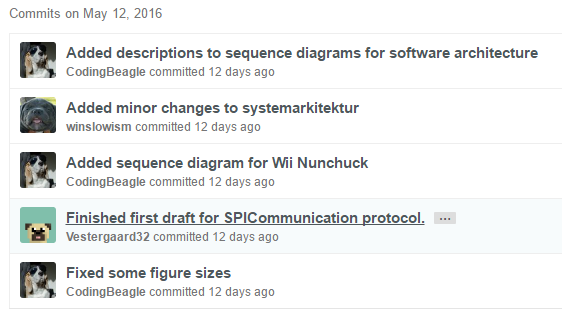
\includegraphics[width=\textwidth]{Projektgennemfoerelse/images/GitHubHistorik}
	\caption{Versionshistorik for et af projektets filer}
	\label{ref:GitHubHistorik}
\end{figure}

\noindent Måden hvorpå gruppen har brugt Git, er at hvert medlem har synkroniseret lokale ændringer løbende til den centrale server. Ved at gøre dette er den nyeste version af projektet altid tilgængeligt for alle andre. \newline

\noindent Git har været en stor hjælp. Det fungerer som en god sikkerhedsmekanisme, da der altid findes en online backup af projektet samt alle ændringer, der er lavet siden begyndelsen. Versionshistorikken er med til at danne et godt overblik over, hvad alle medlemmer arbejder på og retter i. Ved nogle punkter i projektforløbet blev versionshistorikken også brugt til at gendanne tidligere versioner af filer, hvis der ved uheld var introduceret fejl i for eksempel softwarekomponenter. \newline

\noindent Der var dog også komplikationer ved at bruge Git, da alle gruppens medlemmer ikke havde erfaring med det på forhånd. Dette betød at en del tid blev brugt på at lære det. Efterhånden som der blev opnået erfaring med værktøjet, endte det med at være et meget værdifuldt værktøj for projektet.  

\subsection{Pivotal Tracker}
For at have et scrum board på nettet, som alle kunne tilgå blev Pivotal Tracker anvendt. Pivotal Tracker er et professionelt scrumværktøj, der indeholder mange funktioner. Det er blandt andet scrumboardet, grafer over for eksempel burndowncharts og statistikker. Programmet blev valgt ud fra en anbefaling fra vores vejleder.

\textbf{Der skal billeder ind af sprintlog eller lignende} 

\subsection{Facebook}
Til kommunikation mellem gruppensmedlemmer blev der oprettet en Facebook gruppe. Denne gruppe blev brugt til lave aftaler, fildeling og almen kommunikation. Dette værktøj var en essentiel del af gruppe kommunikationen da det er noget som bruges i dagligdagen og det var et værktøj man i forvejen havde kendskab til. \newline

Da der skulle aftales arbejdsdage for påsken blev der oprettet en afstemmning. Med denne afstemmning fik hver medlem tilkendegivet hvilke dage de havde til rådighed. Resultatet af afstemmningen var de to dage der havde størst opbakning. Dette ses i figur \ref{ref:fbpoll}, som er et udsnit af afstemningen.
\begin{figure}[H]
	\centering
	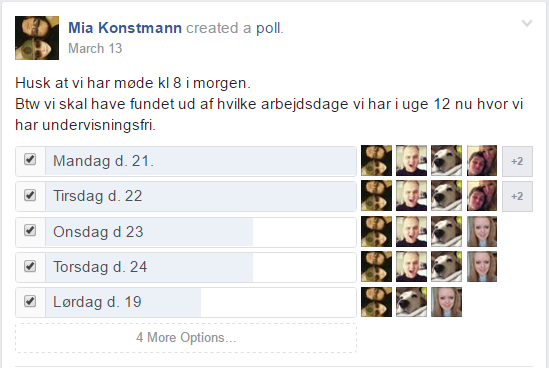
\includegraphics[scale=0.6]{Projektgennemfoerelse/images/fbpoll}
	\caption{Afstemning omkring arbejdsdage}
	\label{ref:fbpoll}
\end{figure}

Facebook gruppen fungerede som en opslagstavle, hvor der kunne dele informationer og meddele hinanden omkring hvordan dokumentation skulle håndteres. Under dette projekt er der blevet brugt LateX til dokumentation. Dermed skulle der lave aftaler omkring hvordan referencer skulle håndteres når det afsnit man refererede til endnu ikke var skrevet. På figur \ref{ref:fblatex} ses at løsningen til dette problem beskrives med en vejledning omkring hvordan referencer skal håndteres.

\begin{figure}[H]
	\centering
	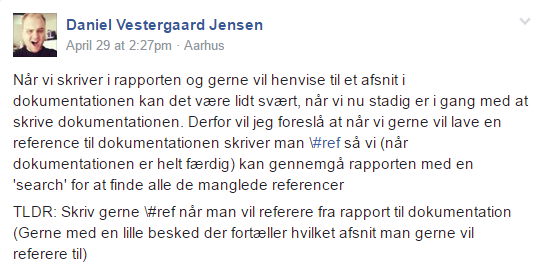
\includegraphics[scale=0.6]{Projektgennemfoerelse/images/fblatex}
	\caption{Opslag omkring referencer}
	\label{ref:fblatex}
\end{figure}

Til at erstatte stå op møderne og logbøger er der blevet oprettet en gruppesamtale. I denne chat informerede man hinanden omkring det der var foretaget dagen før og det der skulle foretages på dagen. Et udsnit af denne samtale ses på figur \ref{ref:fbchat}. Denne form for kommunikation fungerede bedre end de andre forsøg der var blevet gjort i forgående sprint. 

\begin{figure}[H]
	\centering
	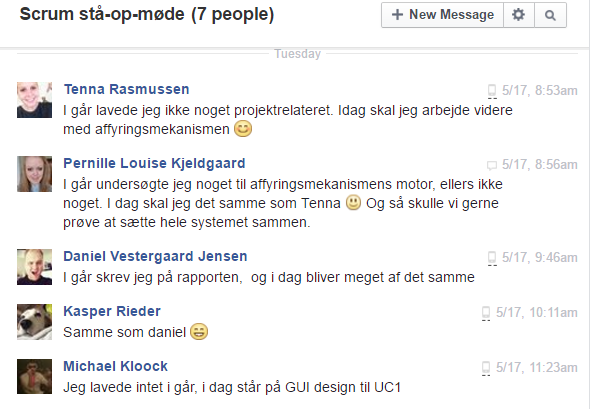
\includegraphics[scale=0.6]{Projektgennemfoerelse/images/fbstandup}
	\caption{Udsnit af gruppesamtalen}
	\label{ref:fbchat}
\end{figure}

Til dette projekt har Facebook været et vigtigt kommunikationsværktøj. Det blev muligt for gruppens medlemmer at kommunikere med hinanden på trods af varierende undervisningstimer og personlige skemaer. Ved at bruge Facebook påmindede man hinanden om at opretholde kommunikationen når man fik en notifikation på sin startside.

\chapter{Scrumkursus ved Systematic}
Som en del af projektet deltog gruppens medlemmer i et scrumkursus som udbydes af Systematic. Som udgangspunkt havde gruppen arbejdet med scrum i to måneder inden kursets start, dermed var der en forforståelse af hvordan scrum skulle anvendes i forbindelse med projekt arbejde. I de følgende afsnit vil de erfaringer som gruppen har gjort sig under kurset.

%\section{Planning Poker}
%En af øvelserne til kurset var planning poker. Her var opgaven at planlægge en flytning, hvor handlingerne for at nå målet skulle tidsestimeres. Under denne øvelse konstaterede gruppen at der var stor uenighed om hvor meget tid der skulle sættes af for at udføre hver delopgave. Der var nogle medlemmer som var optimistiske og forventede at opgaver var hurtigt overstået uden nogle hindringer. Mens der var nogle medlemmer der var pessimistiske og forventede at noget kunne gå galt under udførelsen af opgaverne, som ville forårsage tidsspild. En af opgaverne der skulle planlægges, hvor gruppen var meget uenige i tidsestimeringen, var en teoretisk opgave omkring klargøre et værelse til flytning. Under denne øvelse fik gruppen diskuteret begrundelserne for deres tidsestimeringer og dermed har gruppen fået erfaringer med en alternativ måde at tidsestimere på. Planning Poker er dog ikke blevet brugt under dette projekt forløb, men det har givet værktøjer til at organisere selve tidsestimerings processen.

\section{Scrum Spillet}
En anden af øvelserne til kurset var scrum spillet. Her blev gruppen præsenteret med en backlog af små, veldefineret opgaver. Hver af disse opgaver havde en pointværdi. Når en opgave var fuldført og godkendt af produktejeren, kunne gruppen lægge denne pointværdi til den totale pointsum. Der blev udført tre sprint hver på 15 minutter. Før hvert sprint var der et sprintplanlægningsmøde på 10 minutter og efter hvert sprint var der aflagt fem minutter til retrospective. \newline

Under sprint planlægningsmøderne valgte gruppen de opgaver, som skulle laves i sprintet. Disse kunne enten udføres individuelt eller i grupper, og hvert gruppemedlem meldte sig selv ind på de opgaver de følte de kunne udføre. Dette betød også at hver medlem havde ansvar for de opgaver, som man havde sat sig på og dermed var der en forpligtelse til at udføre opgaven før sprintets afslutning. \newline

Under sprintene var der meget samarbejde omkring arbejdsopgaverne. Når et gruppemedlem konstaterede at der ikke var nok tid til at fuldføre en opgave, blev der hurtigt set på hvilke medlemmer der kunne assistere. Her var gruppen god til at holde overblik og være selvorganiserende. Dette skyldes at kommunikationen fungerede. I modsætning til projektarbejdet, skulle der ikke ydes en indsats for at kommunikere med gruppens medlemmer, da de var omkring en selv. 
I og med opgaverne var veldefinerede, skete der sjældent misforståelser omkring opgavens natur, hvilket betød at arbejdet kunne startes hurtigt. Når der var tvivl omkring opgaverne kunne man konsultere en produktejer som opklarede tvivlen med en klar melding, som gruppen kunne forholde sig til og rette sig efter.  \newline

Til retrospective fik gruppen talt om hvad der fungerede og hvad der ikke fungerede for sprintet. Under første sprint var der ingen struktur omkring hvordan backloggen var sorteret og hvor sprintopgaverne var placeret, hvilket skabte forvirring når der var pres på under selve sprintet. Herefter blev der opsat en struktur i form af lommer der var katagoriseret i \textit{Udførte opgaver} og \textit{Backlog}. I Udførte lommen lå godkendte opgaver og i Backlog så de opgaver der endnu ikke var påbegyndt. Disse opgaver var sorteret, så hurtige og lette opgaver lå øverst og kunne tages hvis der ikke var flere opgaver på sprintbackloggen. De sprintopgaver man havde ansvar på fik man i hånden, så man kunne give den til produktejeren når der skulle godkendes en opgave. \newline
Denne øvelse gav os erfaring med, hvor vigtigt det er at have et organiseret arbejdsrum, og veldefinerede opgaver i forbindelse med scrum og sprints.

\section{Perspektivering}
Under dette kursus har gruppen fået en praktisk forståelse omkring brugen af scrum. Vi oplevede at kommunikationen mellem gruppens medlemmer lykkedes, når vi er fysisk tilstede og har en fysisk og veldefineret sprintbacklog, som vi kan forholde os til. Det ville derfor gavne gruppen at have et grupperum hvor et fysisk scrumboard kunne sættes op. Dermed får vi muligheden for at visualisere de opgaver, der skal udføres i sprintet. \newline
I modsætning til projektarbejdet, var der en ansvarsfølelse for de opgaver der skulle udføres i sprintet. Dette skyldes at vi til scrum spillet valgte opgaver efter vores egne evner og med en sikkerhed om at man kan fuldføre opgaven. Til projektet er arbejdsopgaver valgt med usikkerhed da projektets opgaver omhandler noget man ikke nødvendigvis har kendskab til og er en del af en læringsprocess.

\chapter{Udviklingsforløb}
I bilag \#ref ses en detaljeret beskrivelse af hvert sprintforløb, samt erfaringerne gjort under sprintet.

% \chapter{Opnåede erfaringer}
\chapter{Udfordringer ved anvendelse af scrum}
I forbindelse med at det er første gang, vi anvender scrum til et semester projekt, er der dele af scrum som vi har haft udfordringer med at få inddraget i udviklingsprocessen, hvilket har hindret processen.

\section{Kommunikation}
En vigtig del af scrum er kommunikation. Da gruppen bestod af medlemmer fra forskellige studieretninger, var det ikke muligt at holde daglige morgen møder, hvilket gjorde det uoverskueligt at holde styr på, hvad de andre på teamet lavede. Som kommunikationsværktøj blev der oprettet en Facebook gruppe. Her kunne gruppens medlemmer aftale arbejdsdage og informere hinanden om vigtige ting. Dette værktøj blev ikke anvendt så godt som det kunne have gjort, dermed skete der en del miskommunikation omkring arbejdsdage og hvornår man skulle mødes. \par

\section{Organisering}
Det er ikke muligt for grupper på tredje semester at få et grupperum. Dette ville have gjort en del for kommunikationen at man havde et fællesrum, hvor der kunne arbejdes og hvor scrumboardet kunne placeres. Da dette ikke var en mulighed blev scrumværktøjet Pivitol Tracker anvendt. Der var uklarhed om hvordan dette værktøj skulle anvendes og det tog et par sprint før dette blev afklaret. Her ville det have været en fordel at have et scrumboard med sticky notes, som man arbejder normalt i scrum, eller eventuelt at gøre brug af et mindre kompliceret værktøj til at holde et online scrum-board. Dette kunne for eksempel være Trello eller lignende. 

\section{Sprintbackloggen}
Ved anvendelse af Pivotal Tracker's backlog blev der fra start opstillet en liste af opgaver. I arbejdet med udviklingen af projektet, blev yderligere tilføjelser dog nødvendige. Her har Scrum som agil udviklingsmodel sin fordel, i det, det er muligt at tilføje og ændre i funktionaliteterne for projektet, efterhånden som der opnås yderliger indsigt i behov og muligheder til opnåelse af de opstillede krav. Tidsestimering blev dog, bl.a. som følge af ændringer og tilføjelser, svær at overholde. Her kunne det muligvis have været en fordel at have prioriteret mere tid til sprintplanlægninsmøderne. 

%"Gik galt" er ikke en vending man bruger i en rapport. og afsnit skal skrives løsningsorienteret og ikke som øv bøv verden er træls.

%Anvendelsen af Pivotal Tracker's backlog gik galt fra starten, da der ikke blev lavet en veldefineret liste. For hvert sprint blev der lavet nye opgaver alt efter gruppens ønsker til det kommende sprint. Det at der ikke en veldefineret productbacklog betød at der ikke kunne udvælges opgaver derfra, da disse opgaver ført blev definieret da vi kom i tanke om dem. \par

%Sprintplanlægningsmøderne var præget af en manglende struktur og der blev ikke aflagt nok tid til at afholde disse møder. Dette betød at opgaverne ikke var veldefinerede og disse blev defor ændret i løbet af sprintet, som er noget der ikke må ske under et sprint. Udover at opgaverne ikke var veldefineret, var der opgaver der ikke var taget højde for. Dermed blev der arbejdet på opgaver, der ikke var på sprintbackloggen og tog tid væk fra de tidsestimerede opgaver. Dette førte til at alle opgaver op sprintbackloggen ikke blev fuldtført og tidsplanen blev ved med at skride.

\chapter{Perspektivering}
Processtyringen af dette projekt har været præget af en usikkerhed og uerfarenhed. Dette kan ses i de problemer der er blevet stødt på under projekt forløbet, som for eksempel manglende kommunikation, forhastede planlægningsmøder og fejl i tidsestimeringer. Dette har dog ikke hindret gruppen i at prøve sig frem med nye metoder for at afhjælpe disse problemer. 
For at forbedre kommunikationen mellem gruppens medlemmer blev der forsøgt med forskellige metoder som logbøgerne og morgenmøderne. Vi oplevede dog at dette først blev forbedret da Facebook samtalen blev indført. 
Dette kan 
Der findes utallige metoder til tidsestimering 

Her beskrives hvad der mangler i udviklingsprocessen, og hvad der kan gøres
fremover for at optimere udviklingsprocessen. 